\chapter{Buck-boost equations}\label{ch:Appbuckboost}

The way the buck-boost converter works has been discussed in the introductory chapter \ref{N_INV_BB} The equations that can be used for this type of converter depends on, in which mode the converter are working in. When working in the buck mode the equations below will be used when we see the converter as ideal. 

\section{Buck mode}

The voltages and currents in the different switch stages can be seen in figure \ref{CCM_buck} \todo{needs different pic}

\begin{figure}[htbp]
	\begin{center}
		\includegraphics[width=0.7\textwidth]{../Pictures/CCM_buck}
		\caption{Ideal buck converter in CCM}
		\label{CCM_buck}
	\end{center}	
\end{figure}

Working in CCM mode means that the current through the inductor never falls to zero. When the switch is on(closed) the voltage across the inductor will be: 

\begin{equation}
V_L = V_i-V_o
\end{equation} 

The current through the inductor rises linearly and no current will flow through the diode.
When the switch is off(open) the diode will be forward biased which means the voltage across the inductor will be:

\begin{equation}
V_L = -V_o
\end{equation} 

As seen in the figure \ref{CCM_buck} the current will decrease in this state but never reaches zero.

This equations shows that energy will be stores in the inductor during the on time and decreases in the off time. This means that the inductor is used to transfer the energy from the input to the output of the converter. 
Looking at the voltage part of the figure the yellow surface corresponds to $(V_i-V_o)\cdot t_{on}$ and the orange correndsponds to the $-V_o\cdot t_{on}$. When working in a steady state operation these areas must be equal which in reduced form will be:

\begin{equation}
V_o = D\cdot V_i
\end{equation}

Where $t_{on}=D\cdot T$ and $t_{off}=(1-D)\cdot T$. It can be seen that the output voltage will vary linearly with the duty cycle for a given input voltage.

The current seen at the output will be the average current from both modes:

\begin{equation} \label{Iavg}
I_{Lavg}=I_o
\end{equation}

The ripple current in the inductor can be found with the frequency and inductance:

\begin{equation}\label{buckind}
\Delta I_L = \frac{V_i\cdot D(1-D}{L\cdot f}
\end{equation}
The maximum current ripple through the inductor can be found by looking at the maximum input voltage:

\begin{equation}
\Delta I_{Lmax} = \frac{(V_{imax}-V_{o})\cdot D}{L\cdot f}
\end{equation}

That equation will be used to calculate the peak current in the inductor:

\begin{equation}
I_{Lmax} = I_o + \frac{\Delta I_{Lmax}}{2}
\end{equation}

There are several factors that contribute to the output voltage ripple. Basically the output voltage will rise and fall when the capacitor is charging and discharging. It can be found by calculating $\Delta V_o = \frac{\Delta Q}{C}$, where $\Delta Q$ is the amount of charge. This value is found by integrating $I_L$ from $t_1$ to $t_2$. By doing that $\Delta Q = \frac{\Delta I_L}{8}\cdot T_s$. where $\Delta I_L = (V_o\cdot t_2)/L$ Which means the output voltage ripple can be calculated with:
 
\begin{equation} \label{buckc} 
\Delta V_o = \frac{V_{in}}{8\cdot C_{out}\cdot f^2\cdot L}
\end{equation}    

For the input capacitor the capacitance can be calculated with the equation below:
D
\begin{equation}
\label{buckcin}
C_{in} = \frac{I_o\cdot D\cdot (1-D)}{\Delta V_o\cdot f}
\end{equation}  

\section{Boost mode}
When working in boost mode the output voltage will be larger than the input voltage. The voltages and currents in the different switch stages can be seen in figure \ref{CCM_boost}

\begin{figure}[htbp]
	\begin{center}
		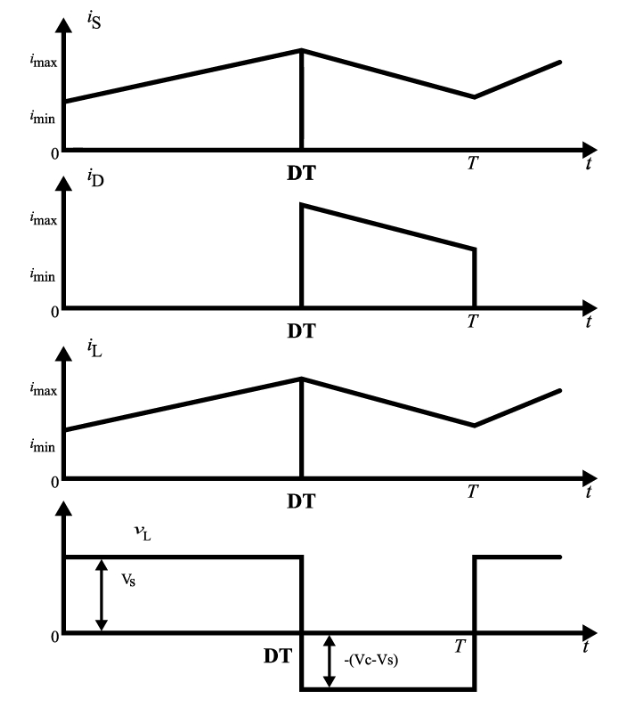
\includegraphics[width=0.7\textwidth]{../Pictures/CCM_boost}
		\caption{Ideal boost converter in CCM}
		\label{CCM_boost}
	\end{center}	
\end{figure}
\todo{picture ref}
In the boost mode CCM will still be used. When the switch is on the voltage across the inductor will be:

\begin{equation}
V_L = V_i
\end{equation}

In this state the inductor current will increase. On the other hand in the off-state the inductor will transfer its energy to the capacitor. Here the voltage across the inductor will be:

\begin{equation}
V_L = V_i-V_o
\end{equation}

In figure \ref{CCM_boost} it can be seen that we are working in CCM because the current never reaches zero. 
When working in steady state the increase of energy stored in the inductor must be equal to the energy transferred to the capacitor during the off state. This means that $\Delta I_{Lon}+\Delta I_{Loff}$. Integrating and reducing these expressions will lead to:

\begin{equation}
V_o = \frac{1}{1-D}\cdot V_i
\end{equation}
 
The average current through the inductor will be calculated as below:
\begin{equation}
I_{Lavg} = \frac{1}{1-D}\cdot I_o
\end{equation}

The ripple current through the inductor can be found using the frequency and the inductance:

\begin{equation}\label{boostind}
\Delta I_L = \frac{V_i\cdot D}{L\cdot f}
\end{equation}
The maximum ripple current through the inductor will be found with the maximum input voltage:
\begin{equation}
\Delta I_{Lmax} = \frac{V_{imax}\cdot D}{L\cdot f}
\end{equation}

With the above equation the peak current through the inductor can be found like this:

\begin{equation}
I_{Lmax} = \frac{1}{1-D}\cdot Io+\frac{\Delta I_{Lmax}}{2}
\end{equation}

 The output voltage ripple can be found by calculating $\Delta V_o = \frac{\Delta Q}{C}$, where $\Delta Q$ is the amount of charge. This value is found by integrating $\frac{-I_o}{c}$ from $D$ to $0$. By doing that the output voltage ripple can be calculated with:

\begin{equation}\label{boostc}
\Delta V_o = \frac{D\cdot I_o}{f\cdot c}
\end{equation}

The input capacitor value can be found with the equation below:

\begin{equation}
\label{boostcin}
C_{in} = \frac{I_o\cdot D\cdot (1-D)}{\Delta V_o\cdot f}
\end{equation}  
